\documentclass[]{article}
% packages
\usepackage{../../cs70}
\usepackage{../../markup}
\usepackage{enumerate}
\usepackage{hyperref}
%% \usepackage{framed}
%% \usepackage{MnSymbol}
%% \usepackage{epstopdf}
\usepackage{color}
%% \usepackage[]{amsmath}
%% \usepackage{graphicx}
%% \usepackage{amssymb}
%% \usepackage{parskip}
%% \usepackage{rotating}
%% \usepackage{float}
%% \usepackage{multirow}
%% \usepackage{subcaption}
%% \usepackage{indentfirst}
%% \usepackage[left=1.5in, right=1.0in, top=1.0in, bottom=1.0in]{geometry}

\newif\ifsolutions
\newif\ifmotivation
\motivationtrue
\motivationfalse
\solutionstrue
\solutionsfalse %flag for solutions

\renewcommand{\answer}[1]{{\color{mydarkblue}\textbf{Solution:}#1}}
\definecolor{mydarkblue}{rgb}{0,0.25,1}

\def\title{Homework 9}

\begin{document}

\maketitle
\config{hwnum}{6}
\config{homework-due}{03/31/2014 13:00}
\config{grades-due}{04/07/2014 13:00}
\vspace{0.5em}
{\Large{\textbf{This homework is due Mar 31 2014, at 12:00 noon.}}}

\begin{qunlist}
  
\qns{Virtual Lab 3: Biased Coins Continued}\\    
In this problem we will continue the lab from last HW. We will start from the optional problem at the end.
\begin{enumerate}[a)]
\qpart 
\item  Up till this point, everything that
  you have done in this virtual lab is something that you could've
  naturally discovered yourself as something worth trying. The data is
  speaking directly to the experimentalist in you. However,
  discovering an actual formula for the shape of this ``cliff-face'' is
  something that actually requires a theoretical investigation that is
  related to counting, Fourier Transforms, and Power Series. Guessing
  its exact shape is not something that comes very naturally on
  experimentalist intuition alone.

  So here, we will simply provide you with the right curve.

  Plot $\int_{-\infty}^d\frac{1}{\sqrt{2\pi}} e^{-\frac{x^2}{2}}dx$
  overlaid with the normalized cliff-face shapes you had plotted in
  the earlier parts. (Do this integral numerically or use the special
  functions that most numerical packages already have for computing
  these sorts of integrals. This integral is related to something
  called the Error Function.) Notice how beautifully it hits the exact
  shape. 

  This is the heart of the Central Limit Theorem as applied to coin
  tosses.

\ifsolutions{ \answer {
\begin{figure}[h!]
\center
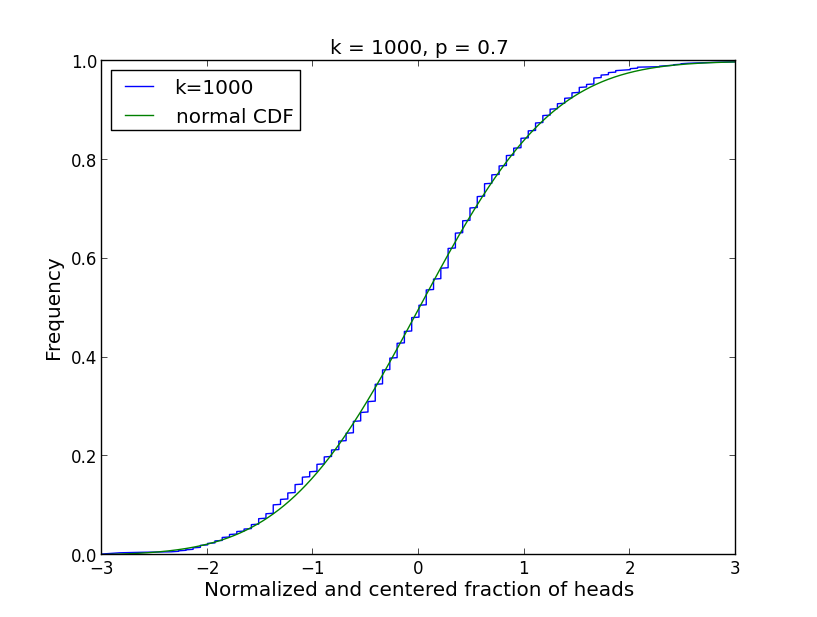
\includegraphics[width=0.5\textwidth]{figs/part_a.png}
\end{figure}
}}\fi

\qpart
\item Just a little notation. We will use $X_i$ to denote a random
  variable that is 1 if you toss a head on the $i$-th toss, and 0 if you toss a
  tail on the $i$-th toss. (This is just so we can more easily express 
  things) So a sequence of $k$ coin tosses would be $X_1, X_2, \ldots,
  X_{k-1}, X_k$, with each $X_i$ being 0 or 1 depending on how the run
  actually came out. How would you write the total number $S$ of heads
  as a function of the $X_i$'s? 

 Our experience from the last homework tells us that the total number
 of heads is itself a random quantity since it varies based on the
 vagaries of the coin tosses.


\qpart 
\item Now, since you had realized earlier that the cliff-faces and the
  histograms have some natural relationship with each other, see if
  you can figure out a way to naturally overlay a smooth plot of
  $\frac{1}{\sqrt{2\pi}} e^{-\frac{x^2}{2}}$ to the normalized
  histograms. What does this mean?

\ifsolutions{ \answer {
\begin{figure}[h!]
\center
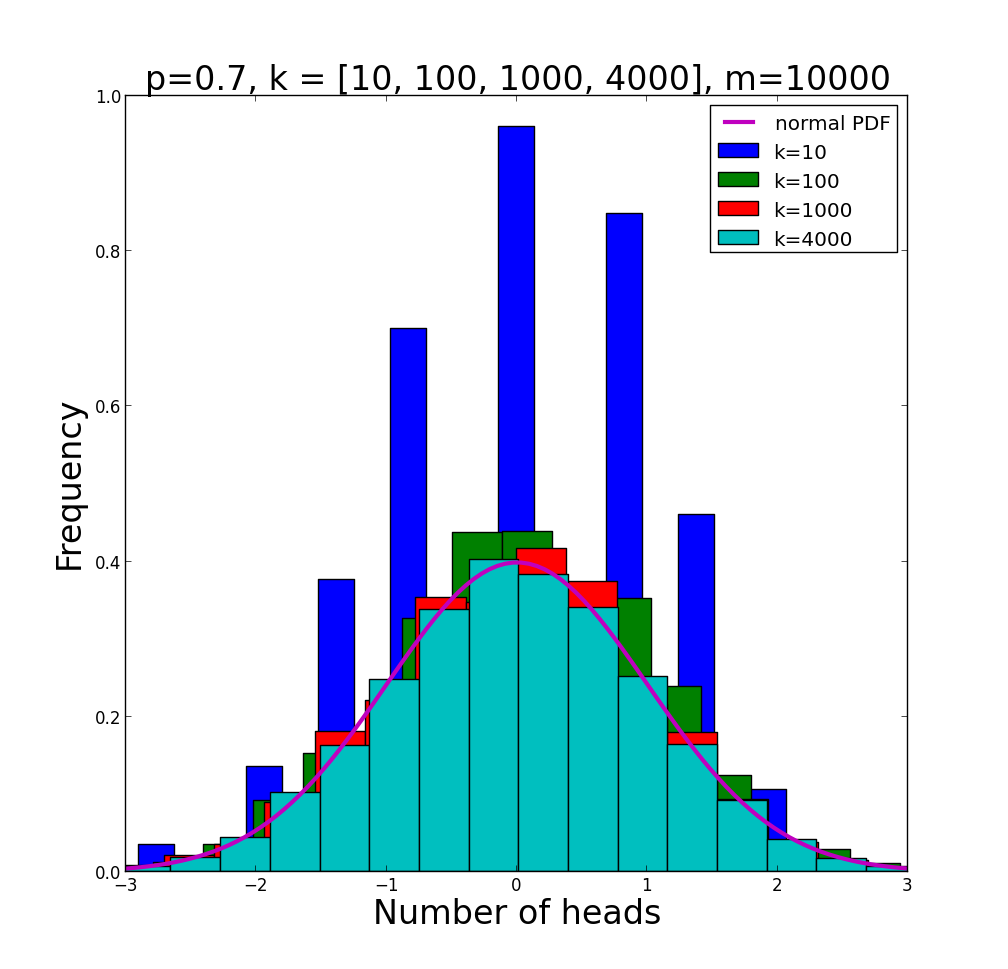
\includegraphics[width=0.5\textwidth]{figs/part_c.png}
\end{figure}
}}\fi

\qpart
\item The other interesting pattern that you had seen in the previous
  virtual lab (In particular, in part k of Q1 on HW7) was the
  exponential drop in the frequencies of certain rare events. For an
  exponential drop, the most interesting thing is to understand the
  rate of the exponential --- or the relevant slope on the Log-Linear
  plot.  

  For a coin with probability $p$ of being heads, we are interested in
  the frequency by which tossing $k$ such coins results in more than
  $ak$ heads (where $a$ is a number larger than $p$). We are
  interested in $p=0.3,0.7$ and $a = p+0.05$,
  $p+0.1$.  Take $m = 10000$ and plot the natural log of the frequencies 
  these deviations against $k$ (ranging from 10 to 200). Approximately
  extract the slopes for all 4 of these.

  Compare them in a table against the predictions of the following
  formula (which we will derive later in the course)
  $$D(a||p) = a \ln \frac{a}{p} + (1-a) \ln \frac{1-a}{1-p}.$$
  
  This expression is called the Kullback-Liebler divergence and is also
  called the relative entropy. 

  Finally, add $e^{-D(a||p) k}$ to the plots (there should be 4 of
  these) you have made as straight lines for immediate visual
  comparison. This straight line is called a ``Chernoff Bound'' on the
  probability in question. 

  Comment. 

\ifsolutions{ \answer {
\begin{figure}[h!]
\center
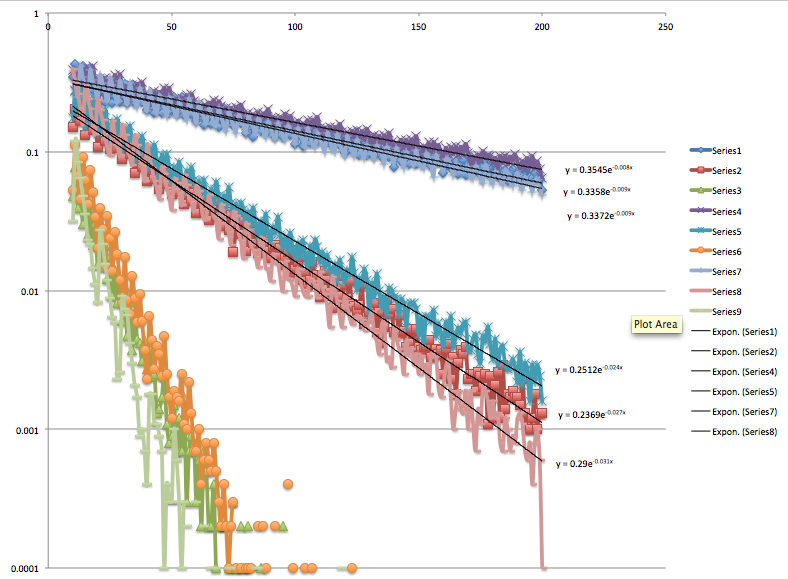
\includegraphics[width=0.5\textwidth]{figs/part_d.png}
\end{figure}
}}\fi

\qpart
\item In the previous part, we went directly to one of the most
  powerful bounds we have. A much simpler bound (that we will
  rigorously derive later in the course) is called Chebyshev's
  inequality. For coin tosses, this inequality says 
$$P(|S_k - k p| \geq \epsilon k) \leq \frac{ p (1-p)}{k \epsilon^2}.$$ 

Notice here that Chebyshev's inequality looks at two-sided
deviations. We count both when $S_k$ is much bigger than $kp$ and when
it is much smaller than $kp$. This is the difference from the previous
bounds. 

We can try to use this for the same kind of big deviations that we had
examined above by trying $\epsilon = 0.1, 0.2, 0.3$. Use simulations to
compare what the actual frequency of such deviations is to what
Chebyshev's inequality estimates.  

Try to make an appropriate plot that shows both Chebyshev's
inequality's prediction and where the actual frequencies are? Why is
this hard?

\qpart
\item Lastly, we would like to explore a function that defines how many ways you can choose $k$ distinct objects out of $n$ possible objects. This is written as $\binom{n} {k}$ and is read aloud as ``$n$ choose $k$''. We define $\binom{n}{k} = \frac{n!}{k!(n-k)!}$ So, for example, $\binom{5}{3} = \frac{5!}{3!(5-3)!} = \frac{5\cdot 4 \cdot 3 \cdot 2 \cdot 1}{(3 \cdot 2 \cdot 1) \cdot (2 \cdot 1)} = \frac{120}{12} = 10$. We wish to explore this function. Plot the value $\binom{50}{k}$ on the $y$-axis and $k$ on the $x$-axis for $0 \leq k \leq 50$.
%Let's try plotting this for $n = 4, 10, 25, 50$.
Does this constantly grow as $k$ gets larger? What does the shape of the graph remind you of?
%You should note a defining feature of the graph. 

\ifsolutions{ \answer {
\begin{figure}[h!]
\center
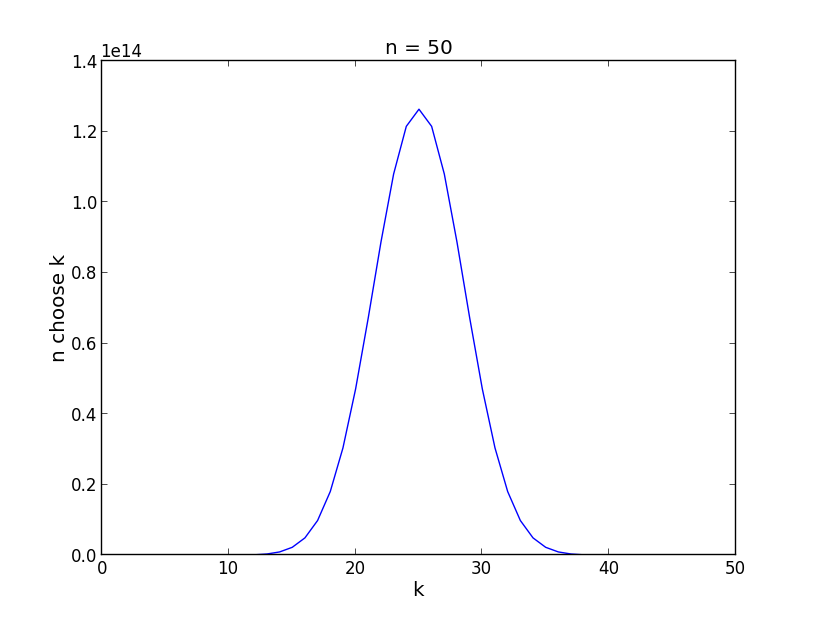
\includegraphics[width=0.5\textwidth]{figs/part_f.png}
\end{figure}
}}\fi

\end{enumerate}



\qns{I'm Hungry... How many Pizzas?}

Suppose that a pizzeria lets me choose toppings for the pizza among $10$ different ingredients. I have budget for buying a pizza with $3$ toppings. For this HW, you may express your answers as expressions, rather than as numbers (for example, $\frac{3!}{5!}$ instead of $0.05$).

\begin{enumerate}[a)]
  \qpart 
\item I choose $3$ distinct toppings. If the order in which I order the toppings matters, (for example: ordering Tomatoes, Onions, Mushrooms is different than ordering Tomatoes, Mushrooms, Onions) how many ways are there to order the toppings?

\ifsolutions{ \answer { 
$10*9*8$

}}\fi
  
  \qpart
\item Now I realize that it doesn't matter what order I ask for the toppings, I still get the same pizza. Again using $3$ distinct toppings out of a possible $10$, how many different types of Pizza can I order?

\ifsolutions{ \answer { 
$\binom{10}{3}$

}}\fi

  \qpart
\item I don't have to get $3$ toppings. If I can instead choose 0, 1, 2, or 3 distinct toppings. For example I could order tomatoes and onions and no third topping. How many different pizzas can I order now?

\ifsolutions{ \answer { 
$\binom{10}{3} + \binom{10}{2} + \binom{10}{1} + \binom{10}{0}$

}}\fi

  \qpart
\item The waiter informs me that I can order repeat toppings (put 2 or 3 portions of the same topping). So now I can order Tomatoes, tomatoes, and onions, for example. Still sticking with my same budget, how many different pizzas can I order, making sure I order exactly $3$ toppings total (although the toppings may not be distinct).

\ifsolutions{ \answer { 
$\binom{10}{3} + 2*\binom{10}{2} + \binom{10}{1}$

}}\fi

\qpart
\item Using the same framework where I can get repeated topping, and not restricting myself to exactly 3 toppings, how many pizzas can I order?

\ifsolutions{ \answer { 
$\binom{10}{3} + 3*\binom{10}{2} + 3*\binom{10}{1} +\binom{10}{0}$

}}\fi

\qpart
\item I go to a cheaper pizzeria, I can now order up to $5$ toppings. How many  pizzas can I buy? (Using the same rules as e above).

\ifsolutions{ \answer { 

$$ \binom{10}{5} +  [1+\binom{4}{1}]\binom{10}{4} +  [1+ 2\binom{3}{1} + \binom{3}{2}] \binom{10}{3} + [1+ 3*\binom{2}{1} + 3*\binom{2}{2}  ]\binom{10}{2} + 5*\binom{10}{1} + \binom{10}{0}$$

}}\fi

\end{enumerate}

\ifmotivation
{\motivation {Motivation - Counting continued but d) is tricky.}}
\fi 


%\qns{Include the stars, exclude the bars}
%
%You are packing for a hike, and you have to choose what to bring with you. You can pick from energy bars, lemons, and bananas. You do not
%want your backpack to be too heavy, so you decide to bring exactly $12$ items with you.
%
%\begin{enumerate}
%  \qpart
%  \item If you have an unlimited supply of each item, in how many ways can you pack your backpack?
%  \qpart
%  \item Now assume that you have $5$ energy bars, $3$ lemons, and $3$ bananas. Now in how many ways can you pack your backpack?
%\end{enumerate}


\qns{Hunger Games}

In this modified version of the book (and movie), Esther is a young adult eligible for tribute to the Hunger Games. Esther is asked to pick 5 cards from a total of 100. Out of these 100 cards, 10 are marked. If at least 1 of the cards out of the 5 Esther picked is a marked card, Esther will go on as tribute to the Hunger Games. 

\begin{enumerate}[a)]
  \qpart
\item How many ways in total are there for Esther to pick 5 out of 100 cards? The order in which she picks these cards does not matter. 
  
  \qpart
\item How many ways can Esther choose the 5 cards such that all are unmarked? Now what is the probability that she will not go on to the Hunger Games? 
  
  \qpart
\item What is the probability that she chooses 5 cards such that 1 is marked and the rest are unmarked? How about the configuration where 2 cards are marked and the rest are unmarked? 
  
  \qpart
\item What is the probability that Esther will go on to the Hunger Games? 
  
  \qpart
\item Given that Esther picked 1 marked card and 4 unmarked cards (she is going to the Hunger Games), her friend Tommy is now forced to choose 5 cards from the remaining pile. Calculate the probability that he will go to the Hunger Games. 
\end{enumerate}

\ifmotivation
{\motivation {Motivation - Basic counting and probability.}}
\fi 

\qns{Clinical Trials}

You are creating a test for a rare disease that only 1 in 1000 people have. If a person has the disease, there is a 95\% chance that your test will be positive.  But if the person does not have the disease, there is only an 85\% chance the test will be negative.

\begin{enumerate}
\qpart 
\item[a)] Let $D$ be the event that you have the disease, and $H$ be the event that you are healthy.  Let $A$ be the event that the test comes out positive, and $B$ be the event that it comes out negative.  Write an expression for $\mathbb{P}(D|A)$ (the probability you have the disease given a positive test result) in terms of the probabilities given above.  Plug in the given probabilities into your expression and calculate the numerical value of $\mathbb{P}(D|A)$.

\ifsolutions{ \answer {
\[ P(D|A) = \frac{P(A|D)P(D)}{P(A)} = \frac{P(A|D)P(D)}{P(A|D)P(D) + P(A|H)P(H)} = \frac{0.95 \cdot 0.001}{0.95 \cdot 0.001 + 0.15 \cdot 0.999} \]
}}\fi

\qpart
\item[b)] Write an expression for $\mathbb{P}(H|B)$, the probability you are healthy given a negative test result.  Evaluate the numerical result of this expression as well.

\ifsolutions{ \answer {
\[ P(H|B) = \frac{P(B|H)P(H)}{P(B)} = \frac{P(B|H)P(H)}{P(B|H)P(H) + P(B|D)P(D)} = \frac{0.85 \cdot 0.999}{0.85 \cdot 0.999 + 0.05 \cdot 0.001} \]
}}\fi

\qpart
\item[c)] For your test to gain approval, the chance of disease given a positive test result must be above 90\%. What would the accuracy of the test have to be to ensure this result?  (You may now assume the accuracy of the test is the same whether you have the disease or not.)

\ifsolutions{ \answer {
Solve for $x$:
\[ P(D|A) = \frac{x \cdot 0.001}{x \cdot 0.001 + (1-x) \cdot 0.999} = 0.9 \] %\quad \Rightarrow \quad x = 99.89\% \]
}}\fi

\end{enumerate}

%\qns{Hunger Games Part 2}
%
%In this again modified version of the book (and the movie), the world is divided into 12 districts, namely District 1 through District 12, and the Capitol. The districts are the colonies of the Capitol, which is run by an evil leader President Snow. The districts have begun to revolt. Powerful President Snow has 20 divisions of indistinguishable robot soldiers. 
%
%\begin{enumerate}[a)]
%  \qpart
%\item How many ways are there for President Snow to send the divisions such that each district has at least 1 division of soldiers?
%  
%  \qpart
%\item Now, President Snow also has a choice to send 0 divisions to districts that do not need soldiers. How many total ways are there for President Snow to divide the 20 divisions?  Sending all 20 divisions to District 1 is different from sending all to District 12. (Hint: represent the distinct outcomes using binary strings. How many of these binary strings are there?)
%\end{enumerate}
%
%\ifmotivation
%{\motivation {Motivation - Stars and Bars problem.}}
%\fi    






\qns{Write your own problem} \\
Write your own problem related to this week's material and solve it. You may still work in groups to brainstorm problems, but each student should submit a unique problem. What is the problem? How to formulate it? How to solve it? What is the solution?

\qns{Midterm question 3} \\
Re-do midterm question 3.
\qns{Midterm question 4} \\
Re-do midterm question 4.
\qns{Midterm question 5} \\
Re-do midterm question 5.
\qns{Midterm question 6} \\
Re-do midterm question 6.
\qns{Midterm question 7} \\
Re-do midterm question 7.
\qns{Midterm question 8} \\
Re-do midterm question 8.
\qns{Midterm question 9} \\
Re-do midterm question 9.
\qns{Midterm question 10} \\
Re-do midterm question 10.
\qns{Midterm question 11} \\
Re-do midterm question 11.
\qns{Midterm question 12} \\
Re-do midterm question 12.
\qns{Midterm question 13} \\
Re-do midterm question 13.
\qns{Midterm question 14} \\
Re-do midterm question 14.
  
  
    
\end{qunlist}


\end{document}
